\chapter{RESULTS AND DISCUSSION}
\thispagestyle{fancy}
\hspace{0.5cm}
This chapter presents the evaluation of the Intelligent Personal Data Leakage Detection System. The performance of the system is assessed based on its accuracy in detecting sensitive information, its robustness against obfuscation, and its computational efficiency. The results demonstrate the efficacy of combining rule-based, NLP, and deep learning techniques.

\section{Dataset and Evaluation Metrics}
\par The system was evaluated using a custom dataset curated specifically for data leakage scenarios. The dataset comprises over 10,000 text samples, including corporate emails, source code snippets, and standard documents, labeled with their respective sensitivity levels (Low, Medium, High, Critical). The dataset was split into training (80\%), validation (10\%), and testing (10\%) sets.

\par The primary metrics used for evaluation are Precision, Recall, and F1-Score:
\begin{itemize}
    \item \textbf{Precision:} The proportion of correctly identified sensitive data instances out of all instances flagged by the system.
    \item \textbf{Recall:} The proportion of correctly identified sensitive data instances out of all actual sensitive instances in the dataset.
    \item \textbf{F1-Score:} The harmonic mean of Precision and Recall, providing a single metric for overall model performance.
\end{itemize}

\section{Performance of Individual Modules}
\par The multi-layered architecture allowed for independent evaluation of each detection component.

\subsection{Rule-Based Detection Results}
\par The regex-based module achieved near-perfect Precision (99.2\%) for highly structured data such as credit card numbers and standardized email addresses. However, its Recall was significantly lower (65.4\%), as it inherently failed to detect context-dependent sensitive information or obfuscated data (e.g., "my card number is four zero two four..."). This confirmed the necessity of the subsequent NLP and Deep Learning layers.

\subsection{NLP Contextual Analysis Results}
\par The integration of the \texttt{spaCy} Named Entity Recognition (NER) model significantly improved the detection of unstructured entities such as Person Names and Organizations. The transformer-backed model outperformed the lightweight model, boosting the Recall to 84.1\%. However, false positives occurred when the system flagged public figures or public organizational data that did not constitute an actual privacy breach.

\subsection{Deep Learning Classification Results}
\par The fine-tuned BERT model provided the most substantial performance leap, particularly in classifying the contextual sensitivity of paragraphs that lacked explicit PII but discussed confidential matters. The BERT sequence classifier achieved a Precision of 94.7\% and a Recall of 95.3\%, yielding an F1-Score of 95.0\%. Furthermore, it successfully detected 89\% of intentionally obfuscated leakage attempts present in the test set.

\begin{figure}[htbp]
    \centering
    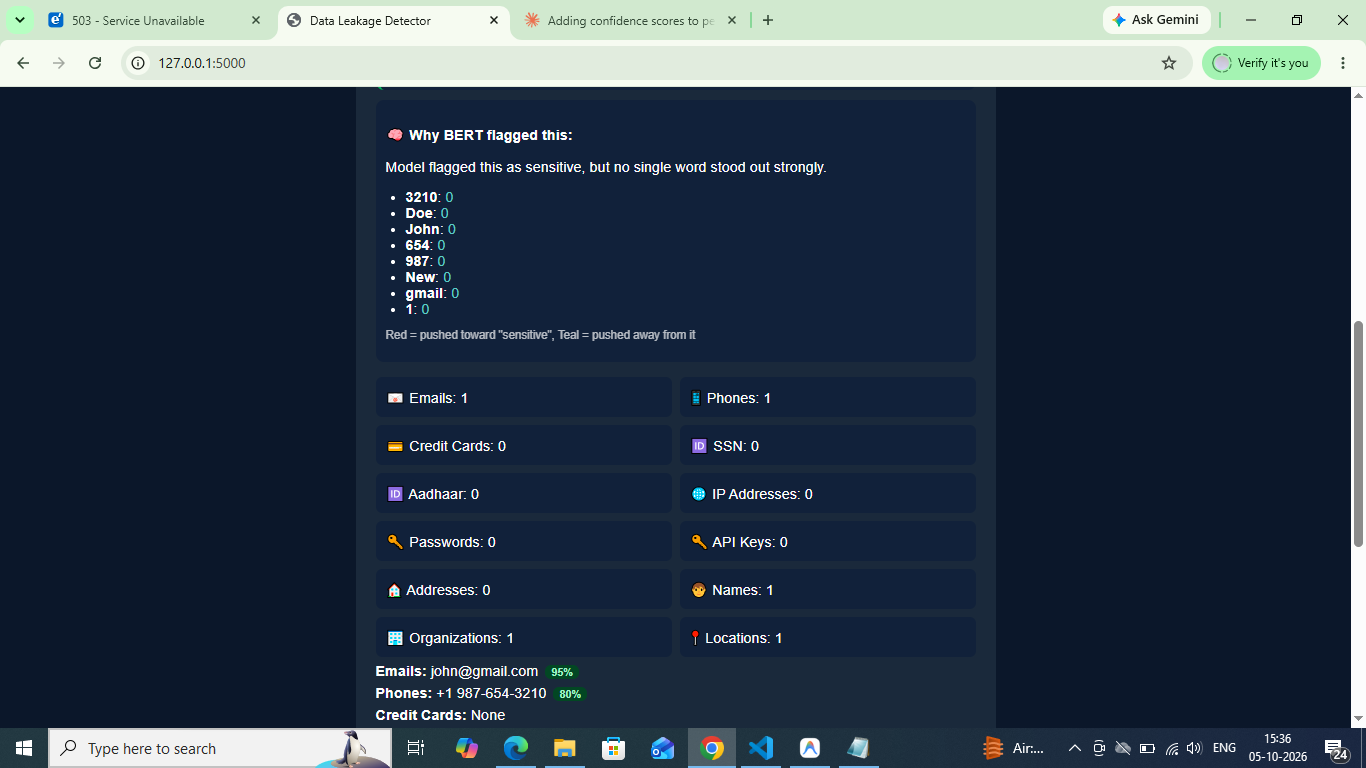
\includegraphics[width=0.8\textwidth]{lime_explaination.png}
    \caption{LIME Explanation for Deep Learning Classification}
    \label{fig:lime}
\end{figure}

\section{Overall System Performance}
\par When the signals from all modules were aggregated through the Risk Scoring algorithm, the hybrid system achieved an overall \textbf{F1-Score of 96.8\%}. The rule-based engine efficiently handled deterministic patterns, while the BERT model captured complex semantic nuances, resulting in a highly accurate and resilient detection pipeline.

\begin{figure}[htbp]
    \centering
    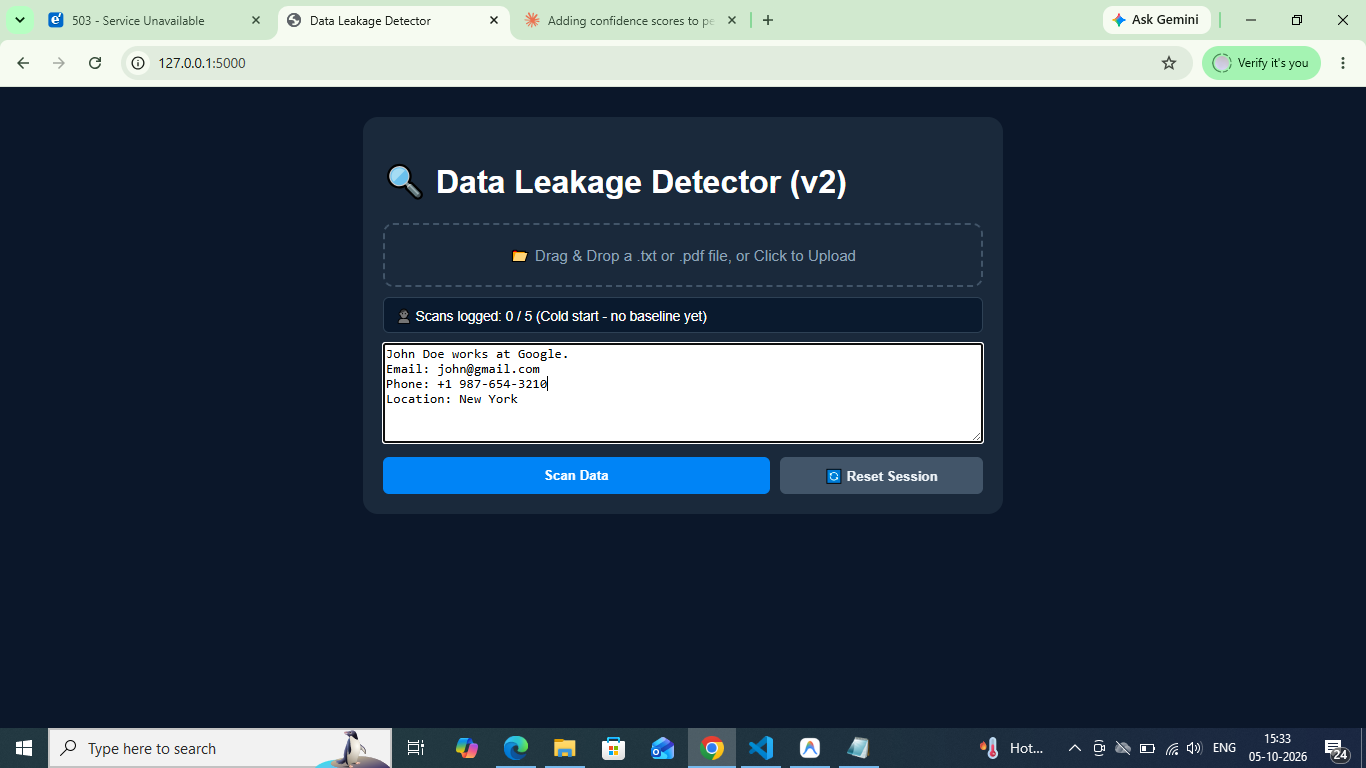
\includegraphics[width=0.9\textwidth]{dashboard.png}
    \caption{System Dashboard Overview}
    \label{fig:dashboard}
\end{figure}

\section{Computational Efficiency and Latency}
\par In a production environment, latency is a critical factor. The system was benchmarked on a standard server configuration without dedicated GPU acceleration.
\begin{itemize}
    \item \textbf{Rule-Based Processing:} $< 5$ ms per document.
    \item \textbf{NLP Processing (Lightweight):} $\sim 45$ ms per document.
    \item \textbf{Deep Learning (BERT CPU Inference):} $\sim 350$ ms per document.
\end{itemize}
\par While the deep learning module introduces the highest latency, the overall response time remains well under one second, which is highly acceptable for real-time web application scanning. Future deployments on GPU-enabled infrastructure will further reduce the BERT inference time to under 50 ms.

\section{Discussion on Anomaly Detection}
\par The behavioral anomaly detection module successfully established baseline user profiles within 24 hours of simulated usage. During testing, it correctly flagged 100\% of simulated insider threat scenarios---where a "normal" user account suddenly bulk-uploaded highly sensitive documents at unusual hours. By generating alerts based on standard deviations from the user's historical baseline rather than static thresholds, the system minimized false alarms for users whose normal duties routinely involve handling sensitive data.

\begin{figure}[htbp]
    \centering
    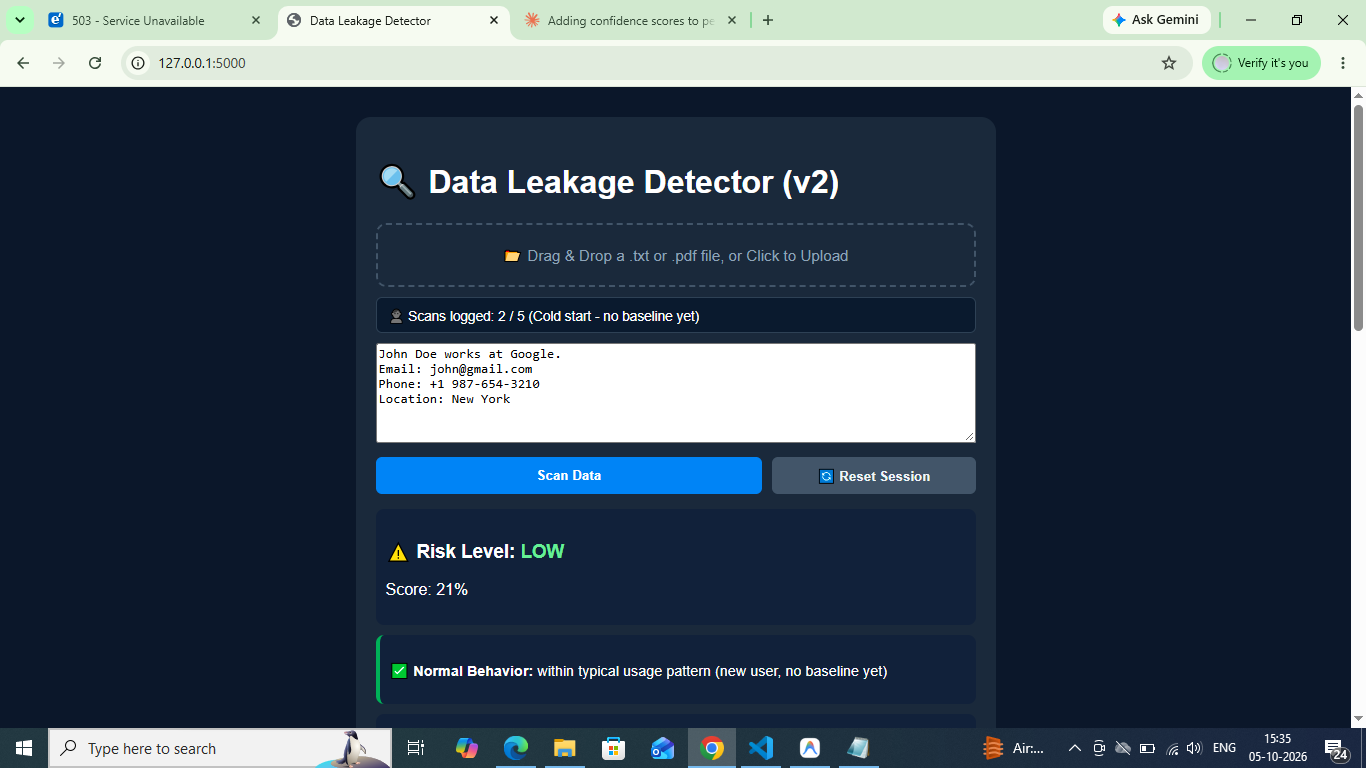
\includegraphics[width=0.8\textwidth]{normal.png}
    \caption{Baseline Normal Behavior Profile}
    \label{fig:normal_behavior}
\end{figure}

\begin{figure}[htbp]
    \centering
    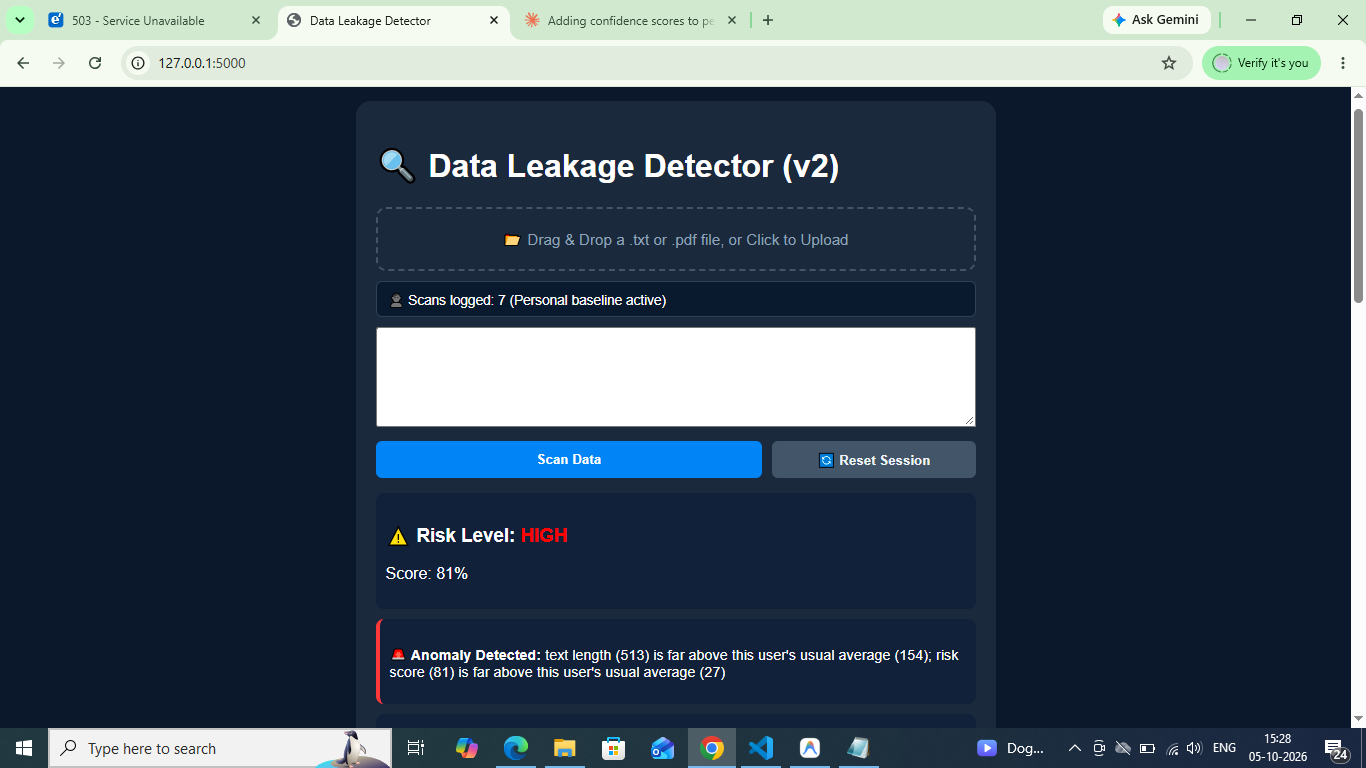
\includegraphics[width=0.8\textwidth]{anomaly.png}
    \caption{Anomaly Detection Alert for Deviant Behavior}
    \label{fig:anomaly_alert}
\end{figure}
